\documentclass[tikz,border=2pt, dvipdfmx]{standalone}
\usetikzlibrary{positioning}

\begin{document}
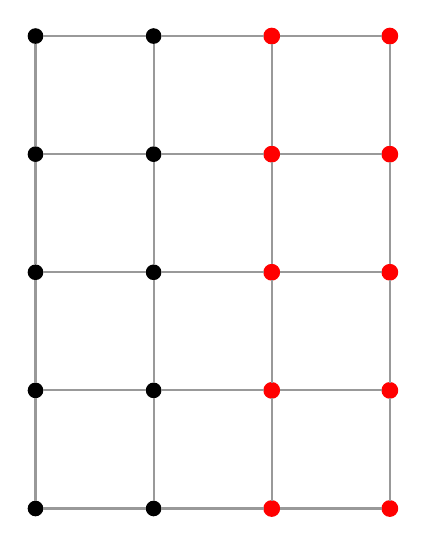
\begin{tikzpicture}[
    node distance=1.5cm and 1.5cm,
    vertex/.style={circle, fill=black, inner sep=2pt, outer sep=0pt},
    red vertex/.style={circle, fill=red, draw=red, inner sep=2pt, outer sep=0pt},
    edge/.style={draw, thick, gray!80}
]
    \foreach \x in {0,...,3} {
        \foreach \y in {0,...,4} {
            \ifnum \x>1
                \node[red vertex] (n-\x-\y) at (\x*1.5, \y*1.5) {};
            \else
                \node[vertex] (n-\x-\y) at (\x*1.5, \y*1.5) {};
            \fi
        }
    }
    \foreach \x in {0,...,3} {
        \foreach \y [count=\ny from 1] in {0,...,3} {
            \draw[edge] (n-\x-\y) -- (n-\x-\ny);
        }
    }
    \foreach \y in {0,...,4} {
        \foreach \x [count=\nx from 1] in {0,...,2} {
            \draw[edge] (n-\x-\y) -- (n-\nx-\y);
        }
    }

\end{tikzpicture}
\end{document}